\documentclass{article}
\usepackage{parskip}
\usepackage{hyperref}
\usepackage{html}
\usepackage[pdftex]{graphicx}
\usepackage{fullpage}
\usepackage{tabularx}
\begin{document}
\title{User Manual}
\author{PLP Dev Team\\
        ECEN \\
        Oklahoma State University, OK}
        
\maketitle
\pagebreak
\tableofcontents

\section{Introduction}
This document serves as the hardware and software developers guide for the 
Progressive Learning Platform (PLP) System on a Chip. The PLP board is a 
unique learning platform designed to be simple, open, and of course, useful 
for education. 
\section{Getting PLP}
Always make sure to download the latest version of PLP. This manual 
reflects the latest version.

PLP is available for download in the 
\htmladdnormallink{downloads}{http://code.google.com/p/progressive-learning-platform/downloads/list}
section. The archive contains the following directory structure:

\begin{enumerate}
\item hw - Hardware images for the CPU
\item sw - Software tools, example programs, and software library
	\begin{enumerate}
	\item PLPTool - PLP Software tools, see next section
	\item libplp - \htmladdnormallink{PLP software library}{http://code.google.com/p/progressive-learning-platform/wiki/libplp}
	\item examples - \htmladdnormallink{Software examples}{http://code.google.com/p/progressive-learning-platform/wiki/SoftwareExamples}
	\end{enumerate} 
\end{enumerate} 

\section{Software Tools (PLPTool)}
PLPTool is a software suite for PLP that includes an assembler, a simulator, 
and a board programmer interface. 
\subsection{Running PLPTool}
PLPTool requires a 
\htmladdnormallink{Java Runtime Environment}{http://www.oracle.com/technetwork/java/javase/downloads/index.html}
that complies with at least Java 2 Platform SE 5 (1.5) specifications. PLPTool 
is shipped with 
\htmladdnormallink{RXTX library}{http://rxtx.qbang.org/wiki/index.php/Main_Page}
for serial communication in Windows. If you use Linux, you will have to 
install the library provided by the distribution that you use. Serial 
communication is used to download programs to the board.

PLPTool is located in \verb+sw/PLPTool+ in the PLP download archive. You 
need to uncompress this folder to run the software. If you use Windows, you 
need to run the batch file \verb+PLPToolWin32.bat+ if you use the 32-bit 
version of Windows, or \verb+PLPToolWin64.bat+ if you use the 64-bit version. 
PLPTool will give a 
warning if it can not detect the RXTX library, and the user will not be 
able to program the board or use the serial terminal. 
\subsubsection{Command Line Options}
Launching PLPTool with no command line arguments will launch the GUI. Launching PLPTool with a \verb+.plp+ file as the only argument will launch the GUI and 
open that project.

\begin{verbatim}
java -jar PLPTool.jar <.plp file to open>
\end{verbatim}

or in Windows, where XX is the CPU type (32- or 64-bit):

\begin{verbatim}
PLPToolWinXX.bat <.plp file to open>
\end{verbatim}

Running PLPTool with the command line argument below will list the source files that are in the project. It will also display the index of said source files that is used to export, remove, or set a source file as top level source.

\begin{verbatim}
java -jar PLPTool.jar -plp <plpfile>
\end{verbatim}

The \verb+-plp <plpfile>+ command can also take additional arguments that can be used to manipulate the project file without launching the GUI: 

\begin{tabular}{ | l | l | }
\hline
Command Line Option & Description \\ \hline
-c \textless asm 1\textgreater  \textless asm 2\textgreater  ... & Creates \textless plpfile\textgreater  and imports \textless asm 1\textgreater , \textless asm 2\textgreater , ... to the project \\
-p \textless port\textgreater  	& Programs \textless plpfile\textgreater  to serial port \textless port\textgreater  \\
-a 	& Performs an assembly of the source files inside \textless plpfile\textgreater  \\
-i \textless asm 1\textgreater  \textless asm 2\textgreater  ... 	& Imports \textless asm 1\textgreater , \textless asm 2\textgreater , ... into \textless plpfile\textgreater  project file \\

-d \textless directory\textgreater  	& Imports all files in \textless directory\textgreater  to the \textless plpfile\textgreater  project file \\
-e \textless index\textgreater  \textless file\textgreater  	& Exports the source file with the index \textless index\textgreater  as \textless file\textgreater  \\
-r \textless index\textgreater  	& Removes the source file with the index \textless index\textgreater  \\
-s \textless index\textgreater  	& Set the source file with the index \textless index\textgreater  as the main program\\

-m \textless index\textgreater  \textless new index\textgreater  	& Set \textless new index\textgreater  for the source file with the index \textless index\textgreater  \\
\hline
\end{tabular}

\subsection{Graphical User Interface}
PLPTool starts in the development environment view, displaying the current open file, files in the project, and a status window. From this view, you can import or create new assembly files, assemble the project, launch the simulator, and program the PLP board. 

\begin{center}
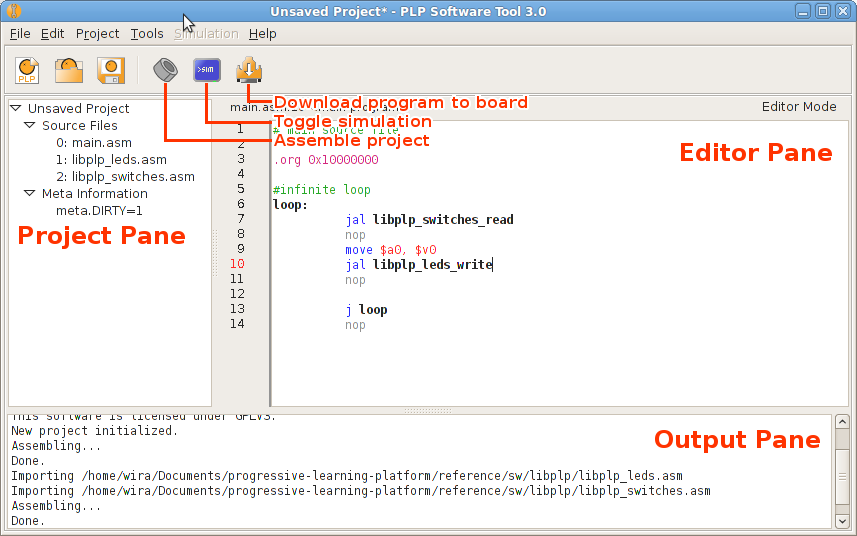
\includegraphics[scale=0.5]{../../images/plptool/plptool30_editor_view.png}
\end{center}

The \textbf{Project Pane} contains all the source files in the project. 
The \textbf{Editor Pane} displays the contents of the currently open source 
file. The \textbf{Output Pane} displays informative, warning, and error 
messages. 
\subsection{Cycle Accurate Simulator}
PLPTool includes a cycle-accurate simulator of the system. This simulator can be accessed from the command-line, or through the graphical user interface. 

\begin{center}
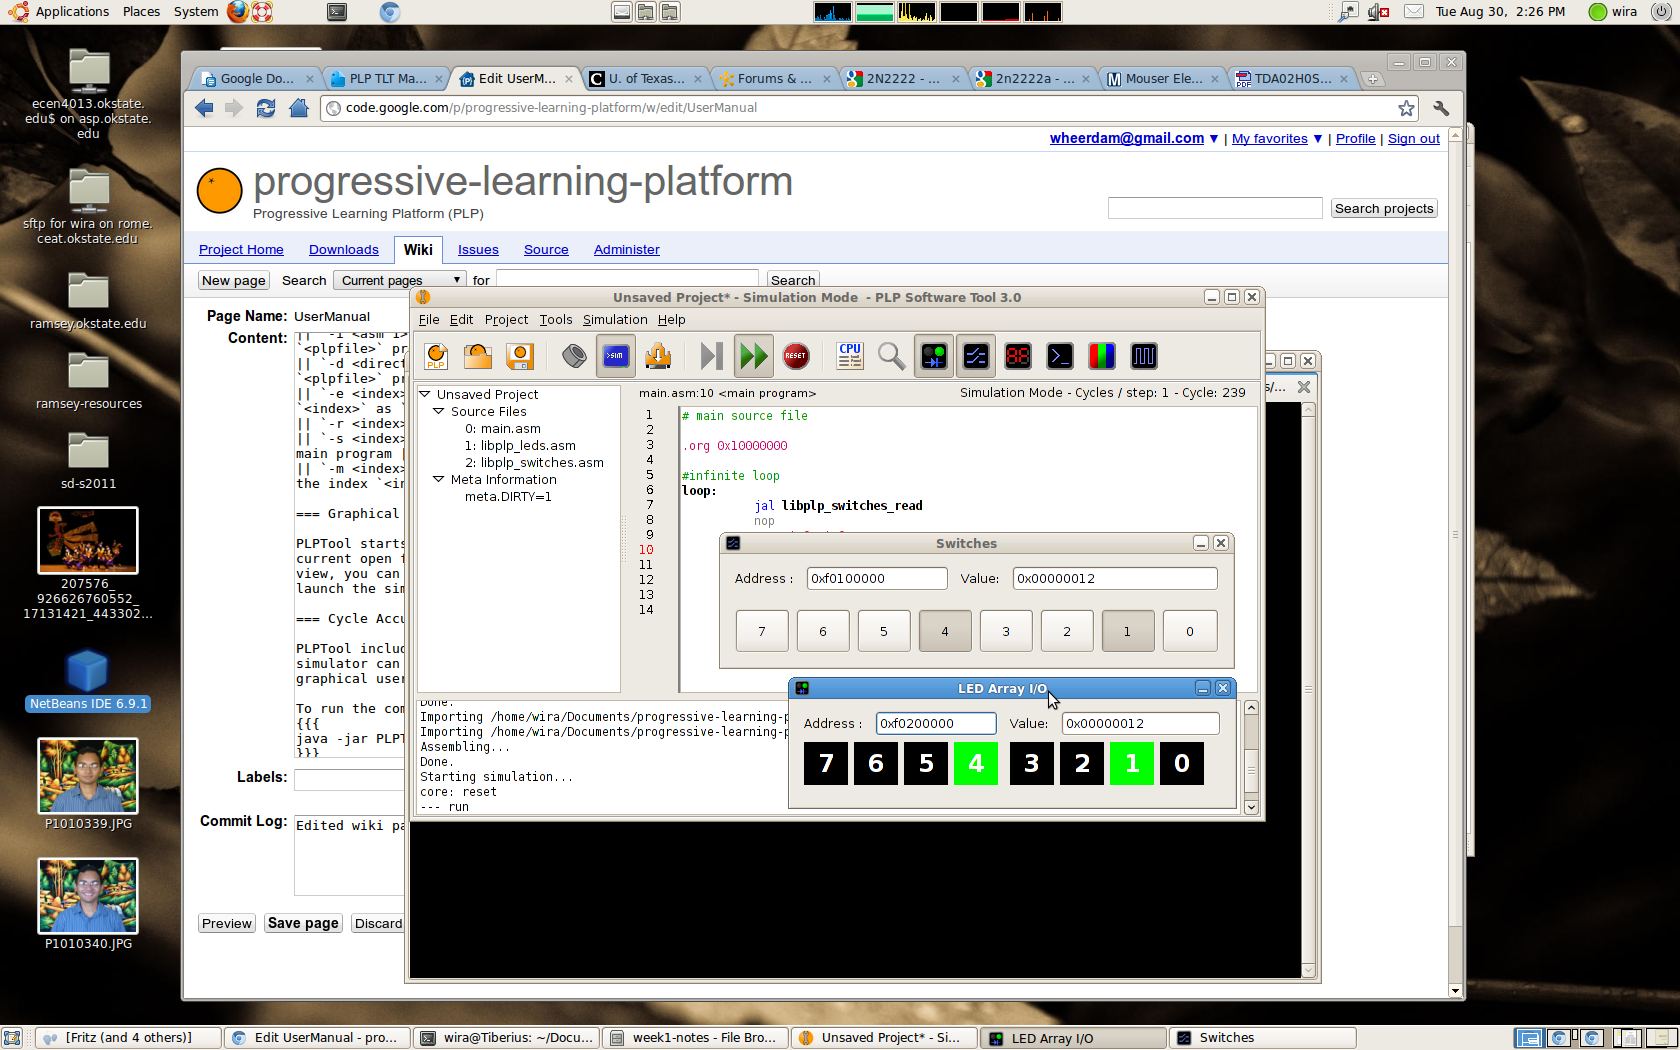
\includegraphics[scale=0.5]{../../images/plptool/plptool30_simulation_mode.png}
\end{center}

The simulation mode adds additional controls to the main window. The first three are the step, run, and reset buttons. Step (F5) will advance the simulation by one cycle, the run toggle button (F7) will continuously run the simulation, and the reset button (F9) will return the CPU to the reset state. The CPU view button will display the CPU window where users can view and modify register file contents, see the disassembly listing, and access the debug console for advanced interaction with the simulation. 
\subsubsection{Setting a Breakpoint}
Breakpoint can be set by double-clicking the line number column. This can only 
applies in lines where there is actually an instruction present. 
Double-click on an existing breakpoint to clear it, or use 
\verb+Tools -> Clear Breakpoints+ to clear ALL breakpoints. 

\subsubsection{Command-Line Mode}
To run the command-line simulator:

\begin{verbatim}
java -jar PLPTool.jar -s <plp file to simulate>
\end{verbatim}
\subsection{Programmer}
You can program the PLP board by selecting 
\verb+Project->Program PLP Board+ 
in the development view. The programmer dialog allows you to select the 
communications port.

Additionally, you can program the PLP board from the command line with:

\begin{verbatim}
java -jar PLPTool.jar -plp <plp project> -p <communications port>
\end{verbatim}
\section{Instruction Set and Assembly Language}
This section describes all supported instructions and pseudo-instructions by the PLP system. It also gives examples on how to use each instruction in a program and notes on limitations. 
\subsection{Syntax}
\subsubsection{Instructions}
Instructions are written in 
\verb+<opcode> <destination>,<operands>+
format, which differ slightly for each type of instruction.

R-type instructions have an opcode and three arguments (either registers or shift amount). For example, to add register 
\verb+$s0+ and \verb+$s1+, 
and store it in register \verb+$t0+, the instruction would be:

\begin{verbatim}
add $t0, $s0, $s1
\end{verbatim}

Shift instructions use the last argument for the shift amount:

\begin{verbatim}
sll $t0, $s0, 5  #shift s0 left 5 bits and store into t0
\end{verbatim}

I-type instructions have two register arguments and an immediate field. For example, to perform a logical OR on 
\verb+$s0+ with the value 0xfeed and store the result in 
\verb+$t0+, the instruction would be:

\begin{verbatim}
ori $t0, $s0, 0xfeed
\end{verbatim}

You may also specify the immediate field in decimal by leaving off the leading '0x'.

Branch instructions require the immediate field to be a label name:

\begin{verbatim}
beq $s0, $s1, loop #if s0 == s1, branch to label "loop"
\end{verbatim}

J-type instructions have only one argument, and must be a label:

\begin{verbatim}
jal my_function #jump and link to label "my_function"
\end{verbatim}

\subsubsection{Pseudo-ops}
PLPTool supports a number of pseudo instructions designed to ease programming and make the assembly more human readable. A list of these instructions, as well as what they map to in the core instruction set is given later in this document. 
\subsubsection{Memory Organization (.org)}
In order to resolve branch and jump targets, the programmer must inform the 
assembler \textbf{before} any instructions, labels, or includes, where the 
program starts in memory. The address must be word aligned (multiple of 4).

\begin{verbatim}
For example, to begin the program at address 0x10000000 (RAM): 
\end{verbatim}

\subsubsection{Labels}
Label support allows the programmer to use branch and jump instructions. Labels are appended with a colon.

For example, to create a label "main": 

\begin{verbatim}
<instructions>
main:
<instructions>
\end{verbatim}

\subsubsection{Comments}
Comments may appear anywhere in the program code, including on label, 
instruction, and directive lines. Comments are prefixed with a \verb+'#'+
character, and all text after the comment character until the end of the line is ignored by the assembler. 

\begin{verbatim}
#a comment on my own line!
add $s0, $s0, $s1 #another comment!
\end{verbatim}

\subsubsection{Data and String Allocation}
There are three ways to allocate space for data with PLPTool: allocating (and optionally initializing) a single word, allocating space in terms of number of words, and by allocating a string. 
\paragraph{Allocate and Initialize Word}
The \verb+.word+ directive allocates a single word with or without an initial 
value. This is especially useful after a label for easy access.

For example, to allocate a variable, initialized to the value 4: 

\begin{verbatim}
my_variable:
.word 4

...

li $t0, my_variable #get a pointer to my variable
lw $t1, 0($t0)      #t1 has my_variable now
\end{verbatim}

\paragraph{Empty Space Allocation}
PLPTool supports allocating space by taking the number of words to allocate, 
as opposed to a single word with the \verb+.word+ directive. This is 
accomplished using the \verb+.space+ directive. For example, to allocate a 
variable with length of 2 words: 

\begin{verbatim}
long_variable:
.space 2

...

li $t0, long_variable #get a pointer to the variable
lw $t1, 0($t0)        #get first word
lw $t2, 4($t0)        #get second word
\end{verbatim}

\paragraph{String Allocation}
PLPTool also supports two types of string allocation
\verb+.ascii, and .asciiz. .ascii+
allocates a packed array of characters without a trailing null 
terminator, which indicates the end of a string.
\verb+.asciiz+ allocates a packed array of characters with a trailing 
null terminator. 

\begin{verbatim}
#a string of characters
my_string:
.ascii "a bunch of characters" #no null terminator here!
#a null terminated string of characters
my_string_null:
.asciiz "a bunch of characters" #null terminated! use me for string operations
\end{verbatim}
PLPTool also supports escaping newline characters with \verb+\n+. 
\subsubsection{Notes on the Assembler}
\verb+.org+ must be the first non-comment statement in the program.

It is possible to load a pointer to a label using the load immediate pseudo instruction (li). 
\subsection{Ops}
\subsubsection{R-type Arithmetic and Logical Instructions}
These instructions receive inputs from two registers, do an arithmetic or logical operation, and write the result in the destination register. The general syntax is: 
\begin{verbatim}
op    $destination_register, $source_register_1, $source_register_2
\end{verbatim}
\begin{tabularx}{\linewidth}{|X|X|X|X|X|}
\hline
Syntax	& C Expression & Sample Usage & Notes & Opcode/Function \\
\hline
addu \$rd, \$rs, \$rt &	rd = rs + rt; &	addu \$v0, \$a0, \$a1 &	Unsigned addition & 0x00 / 0x21 \\
subu \$rd, \$rs, \$rt &	rd = rs - rt; &	subu \$v0, \$a0, \$a1 &	Unsigned subtraction & 0x00 / 0x23 \\
and \$rd, \$rs, \$rt &	rd = rs \& rt; & and \$v0, \$a0, \$a1 &	Bitwise logical AND &0x00 / 0x24 \\
or \$rd, \$rs, \$rt &	rd = rs | rt; &	or \$v0, \$a0, \$a1 &	Bitwise logical OR &0x00 / 0x25 \\
nor \$rd, \$rs, \$rt &	rd = ~(rs | rt); & nor \$v0, \$a0, \$a1 & Bitwise logical NOR & 0x00 / 0x27 \\
slt \$rd, \$rs, \$rt &	rd = (rs < rt) ? 1 : 0;	& slt \$v0, \$a0, \$a1 & Signed compare	& 0x00 / 0x2a \\
sltu \$rd, \$rs, \$rt &	rd = (rs < rt) ? 1 : 0;	& sltu \$v0, \$a0, \$a1	& Unsigned compare & 0x00 / 0x2b \\
mullo \$rd, \$rs, \$rt & rd = (rs * rt) \& 0xFFFFFFFF; & mullo \$v0, \$a0, \$a1	& Multiply (return low order bits) & 0x00 / 0x10 \\
mulhi \$rd, \$rs, \$rt & rd = (rs * rt) \verb+>>>+ 32; & mulhi \$v0, \$a0, \$a1 & Multiply (return high order bits) & 0x00 / 0x11 \\
\hline
\end{tabularx}
\subsubsection{R-type Shift Instructions}
PLP supports logical shift left and right instructions. The general syntax is:

\begin{verbatim}
op    $destination_register, $source_register, shift_amount
\end{verbatim}

Where shift\_amount is a 5-bit integer that can be represented in decimal or hex (with 0x prefix). \textbf{If this value is greater than 5 bits, the assembler will truncate the more significant bit positions beyond the 5th bit place. }

\begin{tabularx}{\linewidth}{|X|X|X|X|X|}
\hline
Syntax & C Expression & Sample Usage & Notes & Opcode/Function \\
\hline
sll \$rd, \$rt, shamt & rd = rt \verb+<<+ shamt; & sll \$v0, \$a0, 0x12 & Shift \$a0 by 18 to the left and store the result in \$v0 & 0x00 / 0x00 \\
srl \$rd, \$rt, shamt & rd = rt \verb+>>+ shamt; & srl \$v0, \$a0, 18 & Shift \$a0 by 18 to the right and store the result in \$v0 & 0x00 / 0x02 \\
\hline
\end{tabularx}
\subsubsection{R-type Jump Register Instructions}
Jump register loads the content of the specified register \$rs into the program counter. 

\begin{tabularx}{\linewidth}{|X|X|X|X|X|}
\hline
Syntax & C Expression & Sample Usage & Notes & Opcode/Function \\
\hline
jr \$rs & PC = rs; & jr \$ra & Load the content of \$ra into PC register & 0x00 / 0x08 \\
jalr \$rd, \$rs & rd = PC + 4; PC = rs; & jalr \$s5, \$t0 & Jump to location specified by the contents of rs, save return address in rd. & 0x00 / 0x09 \\
\hline
\end{tabularx}

\subsubsection{I-type Branch Instructions}
The system supports two branch instructions: branch on equal and branch on not equal. Two registers are compared and appropriate action will be taken depending on the result. The general syntax is: 

\begin{verbatim}
op    $source_register_1, $source_register_2, branch_target
\end{verbatim}

branch\_target has to be a valid label in the program. The assembler takes the address of the label and will calculate the branch offset to be put into the immediate\_field. 

\begin{tabularx}{\linewidth}{|X|X|X|X|X|}
\hline
Syntax & C Expression & Sample Usage & Notes & Opcode \\
\hline
beq \$rt, \$rs, label & if(rt == rs) PC = PC + 4 + imm; & beq \$a0, \$a1, done & Branch to done if \$a0 and \$a1 are equal & 0x04 \\
bne \$rt, \$rs, label & if(rt != rs) PC = PC + 4 + imm; & bne \$a0, \$a1, error & Branch to error if \$a0 and \$a1 are NOT equal & 0x05 \\
\hline
\end{tabularx}

\subsubsection{I-type Arithmetic and Logical Instructions}
These instructions receive inputs from a source register \$rs and the immediate field, and store it in the target register \$rt. The general syntax is: 

\begin{verbatim}
op    $target_register, $source_register, immediate_field
\end{verbatim}

immediate\_field is a 16-bit integer that can be represented in either decimal or hex. \textbf{If this field is greater than 16 bits, the assembler will truncate the more significant bit positions beyond the 16th place.} The processor extends the sign bit of immediate\_field to make it a 32-bit number. 

\begin{tabularx}{\linewidth}{|X|X|X|X|X|}
\hline
Syntax & C Expression & Sample Usage & Notes & Opcode \\
\hline
addiu \$rt, \$rs, imm & rt = rs + SignExtend(imm); & addiu \$v0, \$a0, 0xBEEF & Unsigned addition, add \$a0 with 48879 & 0x09 \\
andi \$rt, \$rs, imm & rt = rs \& ZeroExtend(imm); & andi \$v0, \$a0, 1337 & Bitwise Logical AND & 0x0c \\
ori \$rt, \$rs, imm & rt = rs | ZeroExtend(imm); & ori \$v0, \$a0, 0x0539 & Bitwise Logical OR & 0x0d \\
slti \$rt, \$rs, imm & rt = (rs < SignExtend(imm)) ? 1 : 0; & slti \$v0, \$a0, 0xDEAD & Signed compare & 0x0a \\
sltiu \$rt, \$rs, imm & rt = (rs < SignExtend(imm)) ? 1 : 0; & sltiu \$v0, \$a0, 0xDEAD & Unsigned compare & 0x0b \\
\hline
\end{tabularx}

\subsubsection{I-type Load Upper Immediate Instruction}
This instruction loads the immediate field to the upper 2 bytes of the specified target register. 

\begin{tabularx}{\linewidth}{|X|X|X|X|X|}
\hline
Syntax & C Expression & Sample Usage & Notes & Opcode \\
\hline
lui \$rt, imm & rt = imm << 16; & lui \$a0, 0xBEEF & Write 0xBEEF0000 to \$a0 register. Note that the lower 16 bits are filled with zeroes & 0x0f \\
\hline
\end{tabularx}

\subsubsection{I-type Load and Store Word Instructions}
These instructions read or write data from or to memory. The general syntax is: 

\begin{verbatim}
op    $register, immediate_field($offset_register)
\end{verbatim}

immediate\_field is 16-bit wide and sign extended to 32-bit by the processor to resolve the memory address. If immediate\_field is larger than 16-bit, it will be truncated by the assembler. \$offset\_register acts as an index to the memory address, e.g. an index for an array. 

\begin{tabularx}{\linewidth}{|X|X|X|X|X|}
\hline
Syntax & C Expression & Sample Usage & Notes & Opcode \\
\hline
lw \$rt, imm(\$rs) & rt = SignExtend(imm)[rs]; & lw \$v0, 0x4000(\$a1) & Load contents of 0x4000 + \$a1 into \$v0 & 0x23 \\
sw \$rt, imm(\$rs) & SignExtend(imm)[rs] = rt; & sw \$a0, 128(\$v0) & Store contents of register \$a0 to 128 + \$v0 & 0x2b \\
\hline
\end{tabularx}

\subsubsection{J-type Instructions}
There are two j-type instructions: jump, and jump-and-link. Jump-and-link writes the return address to \$ra when it is called, while jump does not. The syntax is: 

\begin{verbatim}
op    jump_target
\end{verbatim}

jump\_target has to be a valid label. 

\begin{tabularx}{\linewidth}{|X|X|X|X|X|}
\hline
Syntax & C Expression & Sample Usage & Notes & Opcode \\
\hline
j label & PC = jump\_target; & j loop & Jump to loop label & 0x02 \\
jal label & ra = PC + 4; PC = jump\_target; & jal read\_serial & Jump to read\_serial after saving return address to \$ra & 0x03 \\
\hline
\end{tabularx}

\subsection{Pseudo-ops}
The assembler supports a few pseudo-ops to make programming easier. These pseudo-ops are resolved during stage 1 of assembly.

\begin{tabularx}{\linewidth}{|X|X|X|}
\hline
Pseudo-op  &  Equivalent instruction(s)  &  Notes \\
\hline
nop & sll \$0, \$0, 0 & No-operation. Can be used for branch delay slots \\
b label & beq \$0, \$0, label & Branch always to label \\
move \$rd, \$rs & add \$rd, \$0, \$rs & Copy \$rs to \$rd \\
push \$rt & sw \$rt, 0(\$sp); addiu \$sp, \$sp, -4 & Push \$rt into the stack \\
pop \$rt & addiu \$sp, \$sp, 4; lw \$rt, 0(\$sp) & Pop \$rt from the stack \\
li \$rd, imm & lui \$rd, (imm \& 0xff00) \verb+>>+ 16; ori \$rd, imm \& 0x00ff & Load a 32-bit number to \$rd \\
li \$rd, label & lui \$rd, (imm \& 0xff00) \verb+>>+ 16; ori \$rd, imm \& 0x00ff & Load the address of a label to a register to be used as a pointer. \\
\hline
\end{tabularx}

\subsection{Notes on Register Usage}
Aside from \$zero, \$i0, \$i1, and \$ra, the architecture does not explicitly assign special functions to a register. This section lays down some conventions on how the other registers should be used to prevent data from being clobbered across function calls. All the supplied libraries adhere to this guideline. 

\begin{tabularx}{\linewidth}{|X|X|X|}
\hline
Register & Usage & Notes \\
\hline
\$zero	& Constant value 0 & This register can not be written to and always returns the value 0 \\
\$at	& Assembler temporary &	Assembler reserved, do not use \\
\$v0 - \$v1 &	Values for results &	Use for return values of functions \\
\$a0 - \$a3 &	Arguments &	Use for arguments of functions \\
\$t0 - \$t9 &	Temporaries &	Do not use these registers across function calls, as they will most likely be clobbered \\
\$s0 - \$s7 &	Saved temporaries &	- \\
\$i0 &	Interrupt vector &	The CPU jumps to the address pointed by this register when an interrupt occurs \\
\$i1 &	Interrupt return address &	Written by the CPU when an interrupt occurs \\
\$gp &	Global pointer &	- \\
\$sp &	Stack pointer &	Use this register to implement a stack \\
\$fp &	Frame pointer & - \\
\$ra &	Return address & Do not manually write to this register unless restoring from the stack for nested function calls. Use this register to return from a function using the jump register instruction \\
\hline
\end{tabularx}

\section{Hardware Description}
\subsection{Memory Map}
\begin{tabular}{| l | l | l |}
\hline
\textbf{beginning address} & \textbf{length (bytes)} & device \\
\hline
0x00000000 & 2048 & boot ROM \\
0x10000000 & 16777216 & RAM \\
0xf0000000 & 16 & UART \\
0xf0100000 & 4 & switches \\
0xf0200000 & 4 & LEDs \\
0xf0300000 & 12 & GPIO \\
0xf0400000 & 8 & VGA \\
0xf0500000 & 8 & PLPID \\
0xf0600000 & 4 & timer \\
0xf0700000 & 8 & interrupt controller \\
0xf0800000 & ? & performance counter hardware \\
0xf0a00000 & 4 & seven segment \\
\hline
\end{tabular}

\subsection{ROM}
The ROM module is a non-volatile, read-only memory that stores the fload bootloader, which is used with PLPTool to load programs over the serial port. The PLP board starts at address 0x00000000 on power-up and board reset, causing the bootloader to run. 
\subsection{RAM}
The RAM module is a volatile, random access memory that stores all downloaded program code and data. Generally, the programmer will place their program in RAM, beginning at the beginning of RAM using the .org statement (.org 0x10000000). Additionally, the stack is generally initialized at the top of RAM \verb+($sp = 0x10fffffc)+.
\subsection{UART}
The UART module is a UART, running at 57600 baud, with 8 data bits, 1 stop bit, and no parity. The UART module is connected to the serial port on the Nexys 2 development kit.

The UART module is designed to send or receive a single byte at a time, and can only store one byte in the receive buffer. This means that you must read received data (by polling) before the next byte is available.

There are four registers that the UART module uses: 

\begin{tabular}{ | l | l | }
\hline
0xf0000000 & command register \\
0xf0000004 & status register \\
0xf0000008 & receive buffer \\
0xf000000c & send buffer \\
\hline
\end{tabular}

The command register always reads 0. Writing the value 0x01 will initiate a send operation using the lowest byte in the send buffer. Writing a 0x02 will clear the ready flag in the status register.

The status register uses only the bottom two bits, with the remaining bits always reading as 0. status0? is the clear to send bit, which is set after a successful transfer of the data in the send buffer, indicating that another transfer may be made. The cts bit is 0 during a transfer, and the data in the send buffer should not be modified. status1? is the ready bit, which is set when a new byte has been successfully received. The ready bit can be cleared by writing 0x02 to the command register.

The receive buffer holds the last received byte. On a successful receive, the ready bit will be set, allowing the programmer to poll the status register for incoming data. When the ready bit is not set, the receive buffer is considered invalid.

The send buffer holds the byte that will be sent or is ready to send. During a send operation (cts is 0), the data in the transmit buffer must not be modified. Only update the send buffer when cts is set.

The UART supports interrupts, and will trigger an interrupt whenever data is available in the receive buffer. \textbf{The user must complete a receive and clear the status bit in the UART before clearing the interrupt status bit for the UART.}
\subsection{Switches}
The switches module is a read-only register that always holds the current value of the switch positions. There are 8 switches on the Nexys2 development board, which are mapped to the lowest byte of the switches module register. Writing to this location has no effect. 
\subsection{LEDs}
The LEDs module is a read-write register that stores the value of the on-board LEDs. There are 8 LEDs, mapped to the lowest byte of the LED register. Reading this value returns the current LED state, writing will update the LEDs. 
\subsection{GPIO}
The GPIO module connects two of the Nexys2 board's I/O connectors to the PLP system, enabling 16 GPIO ports.

There are three registers that are used with the GPIO module: 

\begin{tabular}{ | l | l |}
\hline
Address & Description \\
\hline
0xf0300000 & Tristate register \\
0xf0300004 & GPIO Block A \\
0xf0300008 & GPIO Block B \\
\hline
\end{tabular}

Each GPIO block on the Nexys2 board has 12 pins: 8 I/O, 2 ground, and 2 Vdd.

The tristate register controls the direction of data on each of the GPIO pins. At startup and on reset, all GPIO are set to be inputs (the tristate register is zeroed). This protects circuits that are driving any pins on the GPIO ports. The user can set GPIO to be outputs by enabling the tristate pins for those outputs. The tristate bits map to GPIO pins in the following table. 

\begin{tabular}{ | l | l |}
\hline
Tristate register bit &	GPIO pin \\
\hline
0 & A0 \\
1 & A1 \\
2 & A2 \\
3 & A3 \\
4 & A4 \\
5 & A5 \\
6 & A6 \\
7 & A7 \\
8 & B0 \\
9 & B1 \\
10 & B2 \\
11 & B3 \\
12 & B4 \\
13 & B5 \\
14 & B6 \\
15 & B7 \\
\hline
\end{tabular}

The GPIO registers use the bottom 8 bits of the data word. The other bits are always read 0. 

\begin{center}
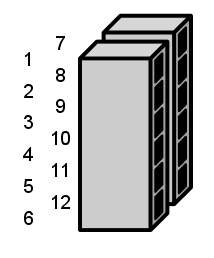
\includegraphics[scale=0.5]{../../images/GPIO.png}
\end{center}

The figure above shows the pin mappings to the below table. 

\begin{tabular}{ | l | l |}
\hline
Pin & Mapping/Bit Position \\
\hline
1 & 0 \\
2 & 1 \\
3 & 2 \\
4 &3 \\
5 & GND \\
6 & Vdd \\
7 & 4 \\
8 & 5 \\
9 & 6 \\
10 & 7 \\
11 & GND \\
12 & Vdd \\
\hline
\end{tabular}

\subsection{VGA}
The VGA module controls a 640x480 display with an 8-bit color depth.

An 8-bit color depth provides 3 red bits, 3 green bits, and 2 blue bits per pixel. The blue channel only has two bits because of a bit-depth limitation as well as the human eye's poor sensitivity to blue intensity. 

\begin{tabular}{ | l | l |}
\hline
bit & color \\
\hline
7 & red[2] \\
6 & red[1] \\
5 & red[0] \\ 
4 & green[2] \\
3 & green[1] \\
2 & green[0] \\
1 & blue[1] \\
0 & blue[0] \\
\hline
\end{tabular}

The VGA module has two registers: 

\begin{tabular}{ | l | l |}
\hline
register & description \\
\hline
0xf0400000 & control \\
0xf0400004 & frame buffer pointer \\
\hline
\end{tabular}

The control register uses only the least significant bit, which enables or disables the VGA controller output. When the control register is 0, the VGA module is disabled. When the control register is 0x1, the VGA module is enabled.

Enabling the VGA module has significant impact on memory performance. The VGA module uses RAM as VGA memory, and has a higher priority to the RAM bus than the CPU. During a draw cycle, the CPU will not be able to access the SRAM for 640 cycles. This effect will be reduced with the inclusion of caches in version 2.2.

The frame buffer pointer is a pointer to the pixel data to draw in memory. For example, if your pixel data begins at 0x100f0000, you would set the frame buffer pointer to that location. The frame buffer must be 0x4b000 bytes long. The pixel data is arranged as starting from the upper left hand corner of the screen (0,0), and drawing to the right, one row at a time (like reading a book). That is, the zeroth pixel in the pixel data is the upper left hand corner. The upper right hand corner is the 639th pixel, and the left most pixel of the second row is the 640th pixel.

A pixel can be indexed by its row and column address (with 0,0 being the upper left hand corner) with : address = base\_address + (640*row) + column 

\subsection{PLPID}
The PLPID module contains two registers that describe the board identity and frequency. Writing to either register has no effect.

0xf0500000 - PLPID (0xdeadbeef for this version) 0xf0500004 - Board frequency (50MHz, 0x2faf080, for the reference design)

The CPUID module is useful for dynamically calculating wait time in a busy-wait loop. For example, if you wanted to wait .5 seconds, you could read the board frequency, shift right by 1 bit, and call the \verb+libplp_wait+ function. 

\subsection{Timer}
The timer module is a single 32-bit counter that increments by one every clock cycle. It can be written to at any time. At overflow, the timer will continue counting. The timer module is useful for waiting a specific amount of time with high resolution (20ns on the reference design).

The timer module supports interrupts, and will trigger an interrupt when the timer overflows. The user can configure a specific timed interrupt by presetting the timer value to N cycles before the overflow condition. 

\subsection{Seven Segment}
\begin{center}
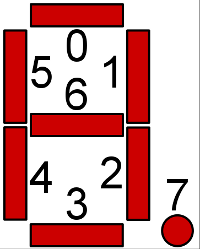
\includegraphics[scale=0.5]{../../images/sseg.png}
\end{center}
The seven segment module exposes the raw seven segment LEDs to the user, allowing for specialized output. libplp wrappers exist for various abstractions.

There are 4 seven segment displays (seven segments plus a dot), mapped to four bytes in the control word.

The byte order is: 

\begin{tabular}{ | l | l | l | l |}
\hline
[31:24] & [23:16] & [15:8] & [7:0] \\
\hline
leftmost & & & rightmost \\
\hline
\end{tabular}

The segments map to each of the four bytes as indicated by the above figure. Bit 0 maps to the top most segment, bit 7 maps to the dot. 

\subsection{Interrupt Controller}

\begin{tabular}{ | l | l | }
\hline
register & description \\
0xf0700000 & mask \\
0xf0700004 & status \\
\hline
\end{tabular}

Status register: 

\begin{tabular}{ | l | l | }
\hline
bit & interrupt reason \\
31-3 & reserved (always 0) \\
2 & UART interrupt \\
1 & timer interrupt \\
0 & always 1 \\
\hline
\end{tabular}

Mask register: 

\begin{tabular}{ | l | l | }
\hline
bit & description \\
31-3 & reserved \\
2 & UART interrupt \\
1 & timer interrupt \\
0 & global interrupt enable \\
\hline
\end{tabular}

The interrupt controller marshals the interrupt behavior of the plp system.

The user uses the two registers in the interrupt controller, mask and status, along with the interrupt registers, \$i0 and \$i1, to control all interrupt behavior.

Before enabling interrupts, the user must supply a pointer to the interrupt vector in register \$i0. 

\begin{verbatim}
main:
  li $i0, isr #put a pointer to our isr in $i0

isr: .
\end{verbatim}
When an interrupt occurs, the interrupt controller sets the corresponding bit in the status register. Before returning from an interrupt the user must clear any status bits that are resolved or unwanted.

The user enables interrupts by setting any desired interrupts in the mask register, as well as setting the global interrupt enable (GIE) bit. When an interrupt occurs, the GIE bit is automatically cleared and must be set on interrupt exit.

\textbf{When returning from an interrupt, set the GIE bit in the delay slot of the returning jump instruction.} This is necessary to prevent any interrupts from occurring while still in the interrupt vector.

When an interrupt occurs, the return address is stored in \$i1.

A typical interrupt vector: 
\begin{verbatim}
isr:
  li $t0, 0xf0700000
  lw $t1, 4($t0)     #read the status register
  
  #check status bits and handle any pending interrupts
  #clear any handled interrupts in $t1

  sw $t1, 4($t0)     #clear any handled interrupts in the status register
  lw $t1, 0($t0)     #get the mask register
  ori $t1, $t1, 1    #set GIE

  jr $i1
  sw $t1, 0($t0)     #store the mask register in the delay slot to guarantee proper exit
\end{verbatim}

\subsection{Performance Counters}
\begin{tabular}{ | l | l | }
\hline
register & description \\
\hline 
0xf0800000 & interrupts \\
0xf0800004 & i-cache misses \\
0xf0800008 & i-cache accesses \\
0xf080000c & d-cache misses \\
0xf0800010 & d-cache accesses \\
0xf0800014 & UART bytes received \\
0xf0800018 & UART bytes sent \\
\hline
\end{tabular}

The performance counter module stores a number of registers that keep count of various events, as shown above. Performance counters are read-only and reset only during board reset. 
\section{Bootloader (fload)}
The PLP board comes with the fload bootloader programmed to the board ROM. fload starts at power-up and reset.

fload currently supports three functions:
\begin{itemize}
\item loading data from the UART
\item memory test
\item memory test with VGA module enabled 
\end{itemize}
These three functions are initiated by setting the appropriate switch after power-up. When all switches are unset, fload will scroll the LEDs indefinitely. When one of the above functions is enabled, only LED 0 will be illuminated.
 
\begin{tabular}{ | l | l | }
\hline
switch & function \\
\hline
0 & UART boot \\
1 & memory test \\
2 & memory test with VGA module enabled \\
\hline
\end{tabular}

The board can be reset at any time by pressing button 0 on the Nexys2 board (or BTNL on the Nexys3). This causes all modules and the CPU to reset, setting the PC to 0. This will restart fload (which resides at address 0x00000000). 
\end{document}
